% \newpage
\chapter*{Введение}                         % Заголовок
\addcontentsline{toc}{chapter}{Введение}    % Добавляем его в оглавление


\section{История вопроса и основные направления}


\subsection{Самоподобное множество}

Геометрическая теория множеств целой и дробной размерности развивается уже более века, при этом множества дробной размерности встречаются и во многих других разделах математики, таких как теория чисел и нелинейные дифференциальные уравнения.
Сильным толчком к изучению таких множеств послужила работа \cite{Man75} Б. Мандельброта  1975 года, в которой  такие множества были применены для описания природных и научных явлений, а также впервые введён термин <<фрактал>>.
Термин <<фрактал>> происходит от латинских fractus (дробный) и frangere (ломать), которыми и описывается суть фрактала как нерегулярного и <<изломанного>> множества.

Мандельброт дал первое определение фрактала как множества, размерность Хаусдорфа которого превосходит топологическую, но он сам признал его неполным.
На практике строго определить фрактал не так просто.
К.~Фальконер \cite{Falconer2004} даёт несколько признаков, которым могут удовлетворять фракталы.
Для того, чтобы можно было назвать объект $A$ фракталом, он должен характеризоваться какими-либо из свойств, перечисленных ниже.

\begin{enumerate}
\item $A$ имеет тонкую структуру, т. е. содержит сложные структурные элементы на любых масштабах;
\item $A$ слишком неоднородно, чтобы описываться на традиционном геометрическом языке;
\item $A$ самоподобно в том или ином смысле, т. е. имеет повторяющуюся структуру в разных масштабах. Возможно, самоподобие приблизительное или статистическое.
\item <<Фрактальная>> размерность (например, размерность Хаусдорфа или клеточная размерность) множества $A$  превышает его топологическую размерность и зачастую является не натуральным числом;
\item $A$ можно построить через рекурсивные или итеративные схемы (что позволяет моделировать фракталы на компьютерах).
\end{enumerate}


Важным разделом фрактальной геометрии является теория самоподобных множеств.
На протяжении всей работы мы будем рассматривать именно самоподобные множества.
Понятие самоподобия упоминается довольно давно, так, например, в 1904 году в своей работе \cite{Koch} Хельге фон Кох строит  непрерывную кривую, не имеющую касательной ни в одной из своих точек, а в 1905 году Чезаро \cite{Ces} указывает на ее самоподобие.
Из более поздних примеров самоподобных множеств можно указать на П. Леви, который в 1939 году \cite{Levy1939} описал самоподобные кривые, состоящие из $n$ копий одинакового размера.

Начало теории самоподобных множеств положил Дж. Хатчинсон в 1981 г. \cite{Hut1981}.
Он дал строгое определение самоподобного множества $K$, являющегося объединением $\bigcup_{i=1}^mS_i(K)$ образов самого себя относительно отображений из системы сжимающих подобий $\eS=\{S_i, i=1,\ldots,m\}$, и описал четкий математический подход к исследованию таких множеств. 
Работа Хатчинсона послужила основой для множества дальнейших исследований.

Прежде всего стоит отметить вклад Р. Молдина и С. Вильямса \cite{MW1988}, которые разработали концепцию граф-ориентированных систем подобий, аттрактором которых является уже система компактов, каждый из которых может состоять не только из своих копий, но и из копий других компактов системы.

В 1996 году М. Моран \cite{Moran1996} определил бесконечно-порождённые самоподобные множества и указал условия, при которых их свойства аналогичны свойствам конечнопорожденных самоподобных множеств.

В теории самоподобных множеств часто возникает вопрос о вычислении фрактальной размерности самоподобного множества.
Под фрактальной размерностью обычно подразумевают одну из нескольких размерностей: размерность Минковского (или т.н. клеточная размерность), упаковочная размерность, размерность Ассуада, размерность Хаусдорфа и некоторые другие.
Для некоторых фракталов эти размерности могут совпадать, но в общем случае они не эквивалентны.

Фрактальная размерность самоподобного множества $K=\bigcup_{i=1}^mS_i(K)$ почти всегда зависит как от коэффициентов подобия $\Lip(S_i)$ отображений системы $\eS$, так и от взаимного расположения и структуры пересечения копий самоподобного множества.
Условия отделимости систем сжимающих подобий, порождающих эти фракталы, помогают определить то, насколько  сильно расположение и  структура пересечений копий самоподобного множества влияют на его фрактальную размерность.
Среди условий отделимости наиболее часто применяются условие открытого множества (OSC) и слабое условие отделимости (WSP).

П.~Моран в 1946 г. \cite{Moran1946} ввел условие открытого множества (OSC) для самоподобных множеств на прямой, а Дж.~Хатчинсон \cite{Hut1981} применил введенное Мораном условие открытого множества к системам сжимающих подобий в $\rr^n$ для любого натурального $n$.

Мы говорим, что система сжимающих подобий $\eS=\{S_1, \ldots, S_m\}$ удовлетворяет условию открытого множества, если существует открытое множество $O$ такое, что множества $\{O_i=S_i(O) | S_i\in\eS\}$ содержатся в $O$ и попарно друг с другом не пересекаются.
Если система $\eS=\{S_1,\ldots,S_m\}$ сжимающих подобий в $\rr^n$ с коэффициентами подобия $r_1, \ldots, r_m$ удовлетворяет условию открытого множества, то хаусдорфова размерность аттрактора этой системы равна его размерности подобия $s$, которая является решением уравнения Морана 
$$r_1^s+\ldots+r_m^s=1.$$ 

Условие открытого множества справедливо далеко не всегда. Но и в случае, когда система $\eS$ удовлетворяет OSC, его проверка может быть сопряжена с определёнными трудностями.
Например, открытое множество может иметь очень сложную структуру или состоять из бесконечного числа связных компонент \cite{AST2024}.
Поэтому К.~Бандт и З.~Граф в 1992 году \cite{SSS7} нашли алгебраический аналог для OSC и ввели алгебраическое условие, основанное на ассоциированном семействе подобий $\mathcal{F}(\eS)$. 
Это условие состоит в том, что $\Id\notin\overline{\mathcal{F}(\eS)}$. Авторы показали, что оно эквивалентно тому, что для  системы $\eS$ с размерностью подобия $s$, $s$-мерная мера Хаусдорфа  ее аттрактора положительна, то есть
$$\Id\notin\overline{\mathcal{F}(\eS)} \Leftrightarrow H^s(K)>0.$$
Более того, при выполнении этого условия пересечения копий самоподобного множества $K$ имеют нулевую меру.

Условие открытого множества можно усилить требованием, согласно которому открытое множество $O$ и аттрактор $K$ системы $\eS$ имеют непустое пересечение. 
Так получается сильное условие открытого множества (SOSC).
В 1994 г. А.~Шиф \cite{Schief1994} показал, что все три условия --- SOSC, OSC и условие положительности меры Хаусдорфа в размерности подобия --- эквивалентны.

Далее, в 1996 году М.~Цернер \cite{Zerner1996} ввёл слабое условие отделимости (WSP).
Самоподобное множество удовлетворяет WSP, если тождественное отображение $\Id$ не является предельной точкой в ассоциированном семействе подобий $\mathcal{F}(\eS)$, то есть $\Id\notin\overline{\mathcal{F}(\eS)}\mmm\mathcal{F}(\eS)$.
Для самоподобных множеств, удовлетворяющих WSP, можно модифицировать уравнение Морана так, что решение этого уравнения будет совпадать с размерностью Хаусдорфа.
Для систем сжимающих подобий, не удовлетворяющих WSP, вычисление размерности Хаусдорфа их аттракторов может быть  непростой задачей.


\subsection{Дендриты}

Далее рассмотрим самоподобные дендриты.
Дендритом называют локально связный континуум, не содержащий простых замкнутых дуг.
Вообще говоря, слово ''дендрит'' является термином из общей топологии \cite{Kur1, Kur2}. Согласно обзору \cite{Char1998} Я. Харатоника и В. Харатоника, история исследований в этой области охватывает более чем 75 лет.

В теории самоподобных множеств с самого ее начала предпринимались попытки выработать некоторые подходы к самоподобным дендритам.
Так в 1985 году М. Хата \cite{Hata1985} показал, что нетривиальный самоподобный дендрит имеет бесконечное множество концевых точек.
В 1990 году К. Бандт показал в \cite{SSS6}, что кратчайшие дуги, соединяющие пары точек самоподобной границы в посткритически конечном самоподобном множестве, являются аттракторами граф-ориентированных систем, а множество возможных значений размерностей таких дуг конечно.
Такие дуги с минимальной размерностью и мерой называются кратчайшими дугами.
В случае самоподобных дендритов, эти результаты описывают главные дуги.

К. Бандт также рассмотрел факторизацию индексного пространства, приводящую к появлению дендритов в \cite{SSS2}.
Дж. Кигами в своей работе \cite{Kig95} применил методы гармонического анализа на фракталах к дендритам. 

В работах последней четверти ХХ века рассматривались несколько важных примеров самоподобных дендритов. К ним можно отнести дерево Хаты \cite{Hata1985}, множество Вичека или пентадендрит \cite{McWorter1987}.
Тем не менее, долгое время отсутствовали удобные геометрические методы, позволяющие целенаправленно конструировать  системы сжимающих подобий, аттракторы которых являлись бы дендритами.
Позднее, в статье \cite{TSV2017}   были описаны методы задания и геометрические свойства самоподобных дендритов в $\rr^d$ --- вопросы, до 2017 года еще недостаточно освещенные в теории самоподобных фракталов. 
Для этого был построен и исследован класс $P$-полиэдральных дендритов в $\rr^d$. 
Такие дендриты $K$ определяются как аттракторы систем $\eS = \{S_1,\ldots, S_m\}$ сжимающих подобий в $\rr^d$, переводящих заданный полиэдр $P \IN \rr^d$ в полиэдры $P_i \IN P$, попарные пересечения которых либо пусты, либо одноточечны и при этом являются общими вершинами  полиэдров $P_i $, а граф попарных пересечений системы полиэдров $P_i$ ацикличен.
Эти же авторы  в работе \cite{STV2017}  более подробно изучили стягиваемые $P$-полигональные системы --- двумерный частный случай $P$-полиэдральных систем  и привели
примеры изоморфизмов между аттракторами двух геометрически различных полигональных систем.
Это привело к поиску более широкого класса дендритов путём ослабления условий, задающих стягиваемые $P$-полигональные системы.
Исследование такого класса дендритов является одной из целей данной работы.

Говоря о полигональных системах, нельзя не упомянуть о полигаскетах, описанных К. Бандтом и Й. Штанке в работе \cite{SSS6} и Р. Стритчартсом в работах \cite{strich1999, Strichartz1999}, которые хоть и не являются дендритами, но для их построения использовались схожие геометрические методы.
Для полигаскетов ими также были описаны кратчайшие дуги, соединяющие пару точек полигаскета и имеющих минимальную размерность и меру.
Кратчайшие дуги позднее будут применены в работах \cite{TSV2017, STV2017} А. В. Тетенова, М. Самуэль и Д. А. Ваулина для построения главных дуг и главного дерева самоподобного дендрита, являющегося аттрактором полигональных систем.

Проверка того, является ли самоподобное множество дендритом, связана со структурой попарных пересечений копий этого аттрактора.
Следует начать с результатов М.~Хаты \cite{Hata1985}, который в 1985 году доказал для самоподобного множества критерий связности.
Опишем эквивалентную формулировку этого критерия.

Рассмотрим для самоподобного множества его граф пересечений, в котором вершинам графа соответствуют копии самоподобного множества, а ребра соединяют вершины, для которых соответствующие копии имеют непустое пересечение.
М.~Хата показал, что самоподобное множество $K$ связно тогда и только тогда, когда его граф пересечений связен. 
При этом, если $K$ связно, то оно локально связно и линейно связно.

В дальнейшем К. Бандт и К. Келлер в работе \cite{SSS2} показали, что если у самоподобного множества копии пересекаются не более чем по одной точке и его граф пересечений есть дерево, то это множество является дендритом. Для дендритов, в которых по одной точке пересекались более двух копий, ими была сформулирована идея двудольного графа пересечений. 
Завершил доказательство этой идеи А. В. Тетенов \cite{FIP}, определив двудольный граф пересечений, в котором одной доле соответствуют копии аттрактора, а другой доле --- точки попарных пересечений этих копий. Ребром в графе могут соединятся только точки разных долей, если соответствующая точка пересечения лежит в соответствующей копии.
Таким образом было получено необходимое и достаточное условие того, что самоподобные множества с одноточечным пересечением являются дендритами.\\


\subsection{Фрактальные квадраты}
\label{ssec:HFS}

Рассмотрим единичный квадрат на плоскости.
Разобьём этот квадрат на $n^2$ равных квадратов с ребром $1/n$, и в этом множестве  квадратов  разбиения выберем какое-то непустое подмножество.
Построим систему $\eS=\{S_1,...,S_m\}$  гомотетий, переводящих единичный квадрат в выбранные  квадраты. Аттрактор $K$ этой системы мы будем называть {\em фрактальным квадратом}.
 Широко известными примерами фрактальных квадратов являются множество Вичека и ковёр Серпинского.


Вообще говоря, фрактальные квадраты являются самоподобным частным случаем самоаффинных {\em ковров Бедфорда-МакМаллена}. 
Последние, в свою очередь, являются двумерным аналогом самоаффинных {\em губок Серпинского}.
Самоподобную губку Серпинского называют фрактальным кубом.


В 1984 году независимо друг от друга Т. Бедфорд \cite{Bedford1984} и К. МакМаллен \cite{McMullen1984} определили и рассмотрели класс самоаффинных множеств, которые впоследствии стали называть коврами Бедфорда-МакМаллена.
Одним из их результатов была формула для вычисления хаусдорфовой размерности   таких множеств.

Как оказалось, размерность и мера ковров Бедфорда-МакМаллена и их многомерных аналогов обладает более сложным поведением по сравнению со своими самоподобными частными случаями.
Так, Ю.~Перес \cite{Peres1994} в 1994 году показал, что мера Хаусдорфа (в своей размерности) у ковров Бедфорда-МакМаллена может быть не $\sigma$-конечной.
Позднее Ю.~Перес и  Р. Кеньон \cite{KenyonPeres1996} вывели формулу хаусдорфовой размерности   для губок Серпинского.
Подробный обзор и сравнение различных фрактальных размерностей (Хаусдорфа, клеточная, упаковочная, Ассуада и др.) для губок Серпинского в 2021 году привёл Дж. Фрейзер \cite{Fraser_2021}.


Так, в 2013 году К.-С. Лау, Дж. Дж. Луо и Х. Рао \cite{LLR2013} рассмотрели топологические свойства замощений плоскости фрактальными квадратами.
Л. Кристеа и Б. Штайнски выпустили цикл работ \cite{CS1,CS2,CS3}, посвящённый выделению и исследованию поддуг во фрактальных квадратах и фрактальных треугольниках.
Они выделили один класс фрактальных квадратов, являющихся дендритами, назвав их лабиринтными фракталами и изучали случайные фракталы, принадлежащие этому классу.
Дж.-Ц. Сяо \cite{Xiao2021} строил и изучал несвязные фрактальные квадраты с конечным числом компонент, для этого он особым образом модифицировал граф пересечений.



\section{Выносимые на защиту положения.}


\begin{enumerate}
\item Доказано, что если аттрактор обобщённой полигональной системы является дендритом, то он удовлетворяет условию совпадения параметров.

\item Доказано, что при достаточно малом $\delta=\delta(\eS)>0$ аттрактор любой (удовлетворяющей условию совпадения параметров) $\delta$-деформации $\eS'$  полигональной системы $\eS$ является дендритом, изоморфным аттрактору системы $\eS$.

\item Доказано, что фрактальные квадраты, являющиеся дендритами, обладают свойством одноточечного пересечения.

\item Доказано, что у фрактальных квадратов, являющихся дендритами, может быть ровно семь возможных топологических типов главного дерева.
\end{enumerate}


\section{Содержание диссертации}


Перейдём к описанию структуры работы и точным формулировкам основных результатов.
Диссертация выполнена в издательской системе \LaTeX, содержит \red{\pageref{LastPage}} страниц и состоит из введения, трёх глав, заключения и списка литературы.
Каждая глава разбита на параграфы.
Список литературы приведён в алфавитном порядке.
Изображения построены в программе IFStile \cite{IFStile} и с помощью макропакета PGF/Tikz для системы \LaTeX.


\textbf{Первая глава} посвящена базовым понятиям теории самоподобных множеств.\\

Дадим определение самоподобного множества. 

\restate{dfn:sss}

Число $q_j=\Lip S_j$ мы называем {\em коэффициентом подобия} отображения $S_j$, для сжимающих подобий $q_j<1$.

Важным и полезным инструментом при описании и изучении самоподобного множества является индексная параметризация копий самоподобного множества.
Пусть дана система $\eS=\{S_1, S_2, \ldots, S_m\}$.
Тогда $I=\{1,2,\ldots,m\}$ --- это {\em множество индексов} системы $\eS$, в то время как $\ia=\bigcup\limits_{n=1}^\8 I^n$ мы называем {\em множеством всех мультииндексов конечной длины} $\bj=j_1 j_2 \ldots j_n$.
Мы говорим, что $\bi\sqsubset\bj$, если  $\bj=\bi\bl$ с некоторым $\bl\in\ia$, то есть слово $\bi$ является началом слова $\bj$. 
Если $\bi\not\sqsubset\bj$ и $\bj\not\sqsubset\bi$, то $\bi$ и $\bj$ называем {\em несравнимыми}.

Для мультииндекса $\bj\in\ia$ мы пишем $S_\bj=S_{j_1j_2\ldots j_n}=S_{j_1}S_{j_2}\ldots S_{j_n}$ и для аттрактора $K=K(\eS)$ мы обозначим $S_\bj(K)$ как $K_\bj$ и будем называть $K_\bj$ {\em копией порядка $n$} самоподобного множества $K$.
Тогда если $\bi\sqsubset\bj$, то $K_\bj\IN K_\bi$.\\

Пусть $\eC:=\{x:\; x\in S_i(K)\cap S_j(K),\; i,j \in I, i\neq j\}$ ---  объединение всех попарных пересечений $S_i(K)\cap S_j(K)$ (при $i\neq j$) копий первого порядка самоподобного множества $K$.
Назовём такое $\eC$ {\em критическим множеством}.
Каждая точка критического множества имеет как минимум два адреса в индексном пространстве.

Множество $\dd K:=\{x\in K: \text{ для некоторого }\bj\in I^* \text{ верно } S_\bj(x)\in \eC\}$ назовём {\em самоподобной границей} для $K$.

Для любой копии $S_\bj(K)$ (при $\bj\in I^*$) мы можем найти множество её граничных точек $\dd K_\bj=\{K_\bj\cap\bigcup\limits_{\bi}K_\bi\ :\ \bi\in I^*,\ \bi\text{ и }\bj\text{ несравнимы}\}$, по которым копия $K_\bj$ пересекается со всеми остальными копиями $K_\bi$ (при несравнимых мультииндексах $\bi$ и $\bj$).
Прообраз $S_\bj^{-1}(\dd K_\bj)$ этого множества граничных точек  содержится в самоподобной границе $\dd K$.\\

На протяжении всей работы особый интерес для меня будут представлять самоподобные множества, являющиеся денритами. 

\restate{dfn:den}

Простой замкнутой дугой мы называем непрерывный иньективный образ окружности.
Дендриты обладают некоторыми примечательными свойствами:
\begin{enumerate}[nolistsep]
\item[1.] Любые две точки дендрита можно соединить единственной лежащей в этом дендрите жордановой дугой;
\item[2.] Любое связное подмножество дендрита само является дендритом;
\item[3.] Пересечение любых связных подмножеств дендрита связно.
\end{enumerate}

Если $K$ --- самоподобный дендрит, то любую пару точек $a_i,a_j\in\dd K$ из его самоподобной границы можно соединить единственной жордановой дугой $\gamma(a_i,a_j)\IN K$.
Такие дуги, соединяющие пары точек самоподобной границы дендрита, мы будем называть {\em главными дугами}.
Если самоподобная граница $\dd K$ самоподобного дендрита конечна, то множество всех главных дуг тоже будет конечно.
Объединение всех главных дуг будем называть {\em главным деревом}.\\

\noindent{\bf Определение \ref{dfn:MT}.}
{\em Пусть $K$ --- самоподобный дендрит c конечной самоподобной границей $\dd K$. 
Минимальный поддендрит $\hat\gamma\IN K$, содержащий $\dd K$, называется {\em главным деревом} дендрита $K$.}\\

Порядок ветвления $Ord(p,X)$ точки $p$ относительно дендрита $X$ совпадает с числом компонент множества $X\setminus\{p\}$.
Точку порядка ветвления 1 мы называем концом, точку с порядком ветвления 2 --- разбивающей, а точку с порядком ветвления не менее 3 --- точкой ветвления.
Заметим, что концами главного дерева $\hat\gamma$ самоподобного дендрита $K$ могут быть только точки из самоподобной границы $\dd K$.
При этом не все точки самоподобной границы $\dd K$ должны быть концами главного дерева $\hat\gamma$.\\

Если в самоподобном множестве его копии попарно пересекаются не более чем по одной точке, то мы говорим, что такое множество обладает свойством одноточечного пересечения.
Для нас интерес представляют как раз самоподобные дендриты с одноточечным пересечением.
Первым удобным класом таких множеств являются аттракторы стягиваемых полигональных систем.

В   работах \cite{TSV2017, STV2017}  такие системы сжимающих подобий определялись следующим образом:

\restate{dfn:cps}

Полигональная система $\eS$ удовлетворяет условию открытого множества (в качестве открытого множества можем взять $\dot P$), если копии аттрактора $K(\eS)$ пересекаются друг с другом не более чем по одной точке, а сам аттрактор является дендритом:

\restate{thm:cpsden}

Среди свойств таких $P$-полигональных дендритов стоит отдельно выделить следующие:
\begin{enumerate}[nolistsep]
\item[1.] $P$-полигональный дендрит $K$ содержится в многоугольнике $P$;
\item[2.] Самоподобная граница $\dd K$ у $P$-полигонального дендрита $K$ совпадает с множеством вершин $\eV_P$.
\end{enumerate}

Если $K$ --- самоподобный дендрит, то любую пару точек $a_i,a_j\in\dd K$ из его самоподобной границы можно соединить единственной жордановой дугой $\gamma(a_i,a_j)\IN K$.
Дуги, соединяющие пары точек самоподобной границы дендриты, мы будем называть {\em главными дугами}.
Если самоподобная граница $\dd K$ самоподобного дендрита конечна, то множество всех главных дуг тоже будет конечно.
Объединение всех главных дуг будем называть {\em главным деревом}.\\

\noindent{\bf Определение \ref{dfn:MT}.}
{\em Пусть $K$ --- самоподобный дендрит c конечной самоподобной границей $\dd K$. 
Минимальный поддендрит $\hat\gamma\IN K$, содержащий $\dd K$, называется {\em главным деревом} дендрита $K$.}\\


Во \textbf{второй главе} получен более широкий класс полигональных дендритов. 
Для этого были ослаблены требования, накладываемые на стягиваемые полигональные системы.

\restate{dfn:gps}

Прежде всего стоит рассмотреть те обобщённые полигональные системы, которые являются $\delta$-деформацией стягиваемой полигональной системы.

\restate{dfn:deform}

Однако аттрактор $K$ обобщённой полигональной системы $\eS$ уже не обязан быть дендритом, поэтому  для $\eS$ требуется дополнительно проверить выполнение условия, задаваемого равенством \eqref{icnd}.\\

\noindent{\bf Теорема \ref{thm:pcint}.}
{\em Пусть $\eS$ --- обобщенная $P$-полигональная система.  
Если для любых $i, j \in I$ 
\begin{equation}
S_i(K)\cap S_j(K)=P_i\cap P_j,\tag{\ref{icnd}}
\end{equation} 
то 
\begin{itemize}[nolistsep]
    \item[(i)] аттрактор $K$ системы $\eS$ является дендритом;
    \item[(ii)] система $\eS$ удовлетворяет OSC;
    \item[(iii)] множество адресов $\pi^{-1}(x)$ всякой точки $x\in K$ конечно.
\end{itemize}}

В таком случае аттрактор $K$ стягиваемой полигональной системы $\eS$ и аттрактор $K'$ её $\delta$-деформации $\eS'$ изоморфны.

\restate{thm:attrmap}

Значит, нам нужно получить условия, при которых аттрактор обобщённой полигональной системы является дендритом с одноточечным пересечением, то есть, выполняется равенство $S_i(K)\cap S_j(K)=P_i\cap P_j$.


Пусть $\eS=\{S_1,\ldots,S_m\}$ -- обобщённая $P$-полигональная система, аттрактор $K$ которой --- дендрит.
Пусть также $A_i,A_j\in V_P$, тогда существует единственная дуга $\Gamma_{ij}\IN K$ с концами в этих точках.
Если $S_i(A_i)=A_i$, то существует дуга $\Gamma\IN\Gamma_{ij}$ с концом в $A_i$ такая, что $S_i(\Gamma)\IN\Gamma$.
Тогда мы говорим, что $\Gamma$ инвариантна относительно подобия $S_i$.

Теперь для любой точки $x=S_i(K)\cap S_j(K)=P_i\cap P_j$ существует пара таких дуг $\Gamma_i\IN K_i$ и $\Gamma_j\IN K_j$, что $\Gamma_i\cap\Gamma_i=x$.
Более того, для этих дуг существуют отображения $S_\bi, S_\bj$ такие, что $S_\bi(x)=S_\bj(x)=x$ и при этом $S_\bi(\Gamma_i)\IN\Gamma_i$ и $S_\bj(\Gamma_j)\IN\Gamma_j$, то есть дуги $\Gamma_i, \Gamma_j$ инвариантны относительно $S_\bi, S_\bj$ соответственно.

Необходимое условие того, что пара таких дуг   пересекается только по общему концу, даёт следующая лемма.

{\bf Лемма о непересекающихся дугах} (см. \cite{ATK}).
{\em Пусть $\Gamma_1$ и $\Gamma_2$ -- такие жордановы дуги с общим началом в $0$ и  концами $z_1$ и $z_2$ ($|z_1|=|z_2|=1$), что $\Gamma_1\cap\Gamma_2=\{0\}$.
Если сжимающие подобия $S_1(z)=\rho_1 e^{i\alpha}z$ и $S_2(z)=\rho_2 e^{i\beta}z$ таковы, что $S_1(\Gamma_1)\IN\Gamma_1$ и $S_2(\Gamma_2)\IN\Gamma_2$, 
а $\alpha:=\Delta\underset{{\Gamma_1\mmm S_1(\Gamma_1)}}{\mathrm {Arg}}(z)$ и $\beta:=\Delta\underset{{\Gamma_2\mmm S_2(\Gamma_2)}}{\mathrm {Arg}}(z)$, то
$$\lambda_1:=\dfrac{\alpha}{\ln\rho_1} = \lambda_2:=\dfrac{\beta}{\ln\rho_2}.$$}

Отношения $\lambda_1$ и $\lambda_1$ мы называем {\em параметрами инвариантных дуг} $\Gamma_1$ и $\Gamma_2$ относительно их общего конца.
Равенство этих параметров является необходимым условием одноточечного пересечения дуг, и мы  его применим для формулировки необходимого условия того, что аттрактор обобщённой полигональной системы является дендритом.

Мы будем говорить, что обобщённая полигональная система система $\eS$ удовлетворяет условию совпадения параметров, если для каждого $x=S_i(P)\cap S_j(P)$ (при $i\neq j$) все инвариантные дуги $\gamma_i\IN S_i(K)$ и $\gamma_j\IN S_j(K)$) с концом в $x$ имеют относительно $x$ одинаковые параметры.

Тогда можно сформулировать первый результат этой главы в следующей теореме.\\

\noindent{\bf Теорема \ref{PMT}} (о совпадении параметров). 
{\em
Пусть аттрактор $K$ обобщенной полигональной системы $\eS$ является дендритом. 
Тогда система $\eS$ удовлетворяет условию совпадения параметров.}

Эта теорема даёт необходимое условие того, что аттрактор обобщённой полигональной системы, в том числе $\da$-деформации, является дендритом. 
Однако даже при соблюдении условия совпадения параметров аттрактор $\da$-деформации может и не быть дендритом, ведь для этого нам нужно, чтобы $\da$ было достаточно малым. 
Оценку для $\da$ даёт наш второй результат этой главы --- теорема о малых деформациях.\\

\noindent{\bf Теорема \ref{mainthm}.} (о малых деформациях)
{\em Для каждой полигональной системы $\eS$ существует такое $\delta > 0$, что для всякой её $\delta$-деформации $\eS'$, удовлетворяющей условию совпадения параметров, аттрактор $K(\eS')$ является дендритом, изоморфным $K(\eS)$.}\\


В {\bf третьей главе} были рассмотрены главные деревья фрактальных квадратов, являющихся дендритами.
В разделе \ref{ssec:HFS} было дано описание фрактального квадрата, определим его более формально.\\

\noindent{\bf Определение \ref{dfn:FS}.}
{\em Пусть $D=\{d_1,\ldots,d_m\}\IN\{0,1,\ldots,n-1\}^2$, где $n\ge 2$, и $1<m<n^2$. 
{\em Фрактальным квадратом} порядка $n$ с {\em множеством единиц $D$} называют компактное множество $K\IN\rr^2$, удовлетворяющее уравнению
$$K=\dfrac{K+D}{n}=\bigcup_{d_i\in D}\dfrac{d_i+K}{n}.$$}

Если у самоподобного дендрита конечная самоподобная граница, то главные деревья таких дендритов имеют конечное число концов.
Тогда мы можем перечислить все топологические типы главных деревьев.
Это позволит разбить все фрактальные квадраты на конечное число классов согласно форме главного дерева.
Значит,  нам нужно рассмотреть структуру самоподобной границы фрактальных квадратов, являющихся дендритами.

Пусть $K=\dfrac{K+D}{n}=K(\eS)$.
Поскольку фрактальный квадрат $K$ содержится в единичном квадрате $P$, \quad $S_i(K)\IN S_i(P)$ для любого $S_i\in\eS$.
Тогда для любых $S_i, S_j\in\eS$ маленькие квадраты $S_i(P)$ и $S_j(P)$ могут пересекаться друг с другом только по общим граням.
Прообразы этих граней в $S_i(P)$ и $S_j(P)$ относительно отображений $S_i$ и $S_j$ соответственно являются парой противоположных граней в квадрате $P$.
Введем  обозначения для граней квадрата $P$ и лежащих в этих гранях точек из фрактального квадрата $K$.

Пусть $A=\{-1,0,1\}^2$. Каждому вектору $\bma=(\al_1,\al_2)\in A$ поставим в соответствие единственную грань единичного квадрата $P=[0,1]^2$ согласно следующему определению.\\

\noindent{\bf Определение \ref{dfn:Pa}.}
{\em Каждый вектор $\bma\in A$ определяет единственную грань $P_\bma$ единичного квадрата $P$ равенством $P_\bma=P\cap(P+\bma)$.}\\

Мы будем говорить, что $\bma\sqsubseteq\bmb$ если и только если $P_\bma\supseteq P_\bmb$, то есть грань $P_\bmb$ является гранью грани $P_\bma$.

 Для фрактального квадрата $K$ его гранью $K_\bma$  называется пересечение $K\cap P_\bma$.
Cогласно Предложению \ref{prop:Ka}, грань $K_\bma$ фрактального квадрата $K$ удовлетворяет уравнению $n K_\bma=K_\bma+D_\bma$, где $D_\bma=D\cap(n-1)P_\bma$, то есть грань $K_\bma$ сама является фрактальным квадратом.

Если для некоторого $\bma\in A\mmm\{0\}$ существуют единицы $d_i,d_i+\bma\in D$, то
$$\dfrac{K+d_i}{n}\cap\dfrac{K+d_i+\bma}{n}=\dfrac{K_\bma+d_i}{n}\cap\dfrac{K_{-\bma}+d_i+\bma}{n}=\dfrac{K_\bma\cap(K_{-\bma}+\bma)+d_i}{n}.$$
Обозначим такое пересечение $K_\bma\cap(K_{-\bma}+\bma)$ пары противоположных граней фрактального квадрата как $F_\bma$.
Тогда для любого $\bma\in A$ верно равенство $K\cap(K+\bma)=F_\bma=F_{-\bma}+\bma $.

Поскольку пересечение $\dfrac{K+d_i}{n}\cap\dfrac{K+d_i+\bma}{n}=\dfrac{F_\bma+d_i}{n}$ содержится в критическом множестве фрактального квадрата $K$,  его прообраз $F_\bma$ относительно $S_i(x)=\dfrac{x+d_i}{n}$ содержится в самоподобной границе $\dd K$.

Для фрактального квадрата $K$ с множеством единиц $D$ мы определим множество $A_D=\{\bma\in A\mmm\{(0,0)\}: D\cap(D+\bma)\neq\0\}$. 
$A_D$ есть множество тех $\bma\in A$, для которых существуют копии $K_i, K_j$ такие, что $d_j-d_i=\bma$.  
Тогда  $K_i, K_j$ могут иметь общие граничные точки, и их общая граница равна $S_i(F_\bma)=S_j(F_{-\bma})$. 
Значит, самоподобная граница $\dd K$ фрактального квадрата $K$ есть объединение
$$\dd K=\bigcup\limits_{\bma\in A_D}F_\bma.$$

Первый результат этой главы выражает пересечение $F_\bma$ через множества $F_\bmb$ (где $\bmb\sqsupseteq\bma$):\\

\noindent{\bf Теорема \ref{thm:falpha}.}
{\em Для $\bma\in A\mmm\{0\}$ множество $F_\bma$ удовлетворяет уравнению
\begin{equation}
F_\bma=\bigcup\limits_{\bmb\sqsupseteq\bma} \dfrac{F_\bmb+G_{\bma\bmb}}{n},\tag{\ref{sideint}}
\end{equation}
где $G_{\bma\bmb}=D_\bma\cap(D_{-\bma}+n\bma-\bmb)$.}\\

Система уравнений \ref{sideint} позволяет найти мощность каждого из множеств $F_\bma$ и, в частности, получить условия, при которых $F_\bma$ будет одноточечным. 
Тем самым мы можем проверить, обладает ли фрактальный квадрат $K$ свойством  одноточечного пересечения.
Следующая теорема даёт условия, при которых множество $F_\bma$ является конечным, счётным или несчётным:\\

\noindent{\bf Теорема \ref{fin_int}.}
{\em Пусть $K=\dfrac{K+D}{n}$ --- фрактальный квадрат и $ \bma\in A$.
\begin{itemize}[nolistsep]
 \item[(i)] Если $\#G_{\bma\bma}> 1$, то множество $F_\bma$ несчётно.
 \item[(ii)] Если $\#G_{\bma\bma}=1$, существует непустое $F_\bmb$ при $\bmb\sqsupset\bma$ и $\#G_{\bma\bmb}\geq1$, то $F_\bma$ бесконечное счётное.
 \item[(iii)] Множество $F_\bma$ конечно в следующих случаях:
 \begin{itemize}[nolistsep]
 \item[\textbf{(a)}] $\#G_{\bma\bma}=1$ и $\#F_\bmb\cdot\#G_{\bma\bmb}=0$ для каждого $\bmb\sqsupset\bma$;
 \item[\textbf{(b)}] $\#G_{\bma\bma}=0$ и существует $\bmb\sqsupset\bma$ такое, что $\#F_\bmb\cdot\#G_{\bma\bmb}\geq1$.
 \end{itemize}
\end{itemize}}\medskip

Из этой теоремы  получаем условия, при которых $F_\bma$  одноточечно:

\noindent{\bf Следствие \ref{onepoint}.}
{\em Множество $F_\bma$ одноточечно, если \\
\textbf{(a)} $\#G_{\bma\bma}=1$ и $\#F_\bmb\cdot\#G_{\bma\bmb}=0$ для каждого $\bmb\sqsupset\bma$; или\\
\textbf{(b)} $\#G_{\bma\bma}=0$ и существует $\bmb\sqsupset\bma$ такое, что $\#F_\bmb\cdot\#G_{\bma\bmb}=1$.}\smallskip

Далее мы рассмотрим второй результат текущей главы.
\\

\noindent{\bf Предложение \ref{thm:den_necessary_sufficient}.}
{\em Если фрактальный квадрат $K$ является дендритом, то он обладает свойством одноточечного пересечения.}\\

Из этого следует, что фрактальный квадрат $K$ является дендритом тогда и только тогда, когда его двудольный граф пересечений является деревом.

Поскольку для любого $\bma\in A\mmm\{0\}$ множество $F_\bma$ не более чем одноточечно,   самоподобная граница $\dd K$ также конечна.
Следующая теорема группирует фрактальные квадраты, являющиеся дендритами, по типам в зависимости от расположения точек их самоподобной границы.\\

\noindent{\bf Теорема \ref{ssboundary}.}
{\em Пусть $K$ --- фрактальный квадрат, являющийся дендритом и не являющийся отрезком.
Тогда $\#\dd K\in\{3,\ 4,\ 6\}$. \\

Если $\#\dd K=4$, то  $\dd K=F_\bma\cup F_{-\bma}\cup F_\bmb\cup F_{-\bmb}$, где   пара  $\bma,\bmb$ принимает одно из следующих значений:
	\begin{itemize}
	\item[{\bf A.}] $\bma=(1,0)$, $ \bmb=(0,1)$;
	\item[{\bf B.}] $\bma=(1,1)$, $ \bmb=(1,-1)$;
	\item[{\bf C.}] $\bma\in\{(1,1),\ (1,-1)\},\bmb\in\{(1,0),\ (0,1)\}$.
	\end{itemize}
Если $\#\dd K=3$ или $\#\dd K=6$, то 
\begin{itemize}
	\item[{\bf D.}] $\dd K=F_{(1,0)}\cup F_{(-1,0)}\cup F_{(0,1)}\cup F_{(0,-1)}\cup F_\bmb\cup F_{-\bmb}$, где $\bmb\in\{(1,1),\ (1,-1)\}$.
\end{itemize}}

Точки самоподобной границы таких дендритов нужно рассмативать парами, поскольку если $F_\bma\in \dd K$, то и $F_{-\bma}\in \dd K$,  причём $F_{\bma}=F_{-\bma}+\bma$.
Значит, во фрактальном квадрате типа {\bf A} пары таких точек $\dd K$ лежат в парах противоположных рёбер.
Для типа {\bf B} точки из $\dd K$ лежат в угловых точках единичного квадрата $P$.
Для типа {\bf С} точки из $\dd K$ лежат в одной паре противоположных рёбер и в одной паре противоположных углов квадрата $P$.
И, наконец, для типа {\bf D} точки из $\dd K$ лежат либо в обеих парах противоположных рёбер и в одной паре противоположных углов квадрата $P$, либо в трёх угловых точках квадрата $P$.

Теперь, зная мощность самоподобной границы фрактальных квадратов, являющихся дендритами, мы можем перечислить все топологические типы их главных деревьев.
Поскольку $\#\dd K\leq6$,  в главном дереве не может быть более 6 концов.
Это даёт нам 13 возможных конфигураций главного дерева, но не все из них будут возможны.
Чтобы определить действительные конфигурации главного дерева, рассмотрим следующие вспомогательные результаты.

Лемма \ref{thm:vertex_branching} говорит о том, что если $K$ --- фрактальный квадрат, являющийся дендритом, то для любой угловой точки $a\in K$ её порядок ветвления $Ord(a,K)\leq 2$.
Их этой теоремы есть следствие, по которому во фрактальных квадратах типа {\bf B} и {\bf D3} порядки ветвления угловых точек равны 1.
Это не позволяет сделать одну из угловых точек самоподобной границы точкой ветвления, а также говорит о точ, что главные деревья фрактальных квадратах типа {\bf B} и {\bf D3} имеют 4 конца.

Теорема \ref{order} порядок ветвления любой точки $x$ фрактального квадрата $K$, являющегося дендритом.
Так для любого  $x\in K$ верно $Ord(x,K)\le 4$, а если $K$ относится к типу {\bf D3}, то $Ord(x, K)\le 3$.
Это позволяет отсеять деревья с точками ветвления порядка 5 и 6, а также допускает для фрактального квадрата типа {\bf D3} единственный тип главного дерева --- дерево с тремя концами и точкой ветвления порядка 3.

Теорема \ref{lem:d4bound} рассматривает фрактальные квадраты $K$ типа {\bf D6}.
Тогда если $\gamma$ ---  главное дерево для $K$, то
\begin{itemize}[nolistsep]
    \item[(i)] $Ord(x,\gamma)\leq2$ для любого $x\in\dd K$;
    \item[(ii)] $Ord(x,K)\leq3$ для любого $x\in\ga$.
\end{itemize}
Эта теорема исключает деревья с 5 и 6 концами, имеющие точки ветвления порядка 4.

Теперь мы можем сформулировать последний результат главы.\\

\noindent{\bf Теорема \ref{thm:7trees}.}
{\em Для фрактальных квадратов, являющихся дендритами, существует только $7$ топологических типов главного дерева, модели которых показаны ниже.}
\begin{figure}[H]
    \centering \Large {\bf
    1. 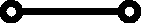
\includegraphics[width=0.15\textwidth]{mt1.pdf}
    \hfill
    2. 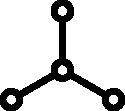
\includegraphics[width=0.15\textwidth]{mt2.pdf}
    \hfill
    3. 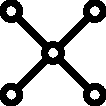
\includegraphics[width=0.13\textwidth]{mt3.pdf}
    \hfill
    4. 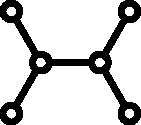
\includegraphics[width=0.15\textwidth]{mt4.pdf}\\
    \bigskip
    5. 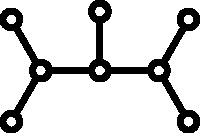
\includegraphics[width=0.23\textwidth]{mt5.pdf}
    \hfill
    6. 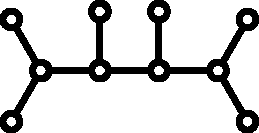
\includegraphics[width=0.3\textwidth]{mt7.pdf}
    \hfill
    7. 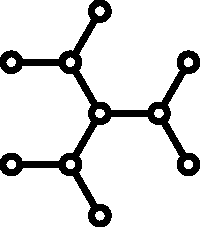
\includegraphics[width=0.22\textwidth]{mt6.pdf}}
\end{figure}

Таким образом, если мы будем классифицировать фрактальные квадраты, являющиеся дендритами, по форме главного дерева, то мы получим 7 классов фрактальных квадратов.

Если принять во внимание гипотезу о том, что во фактальном квадрате типа {\bf D6} число концов в его главном дереве $\gamma$ не меньше 4, то мы можем рассмотеть {\em тонкую классификацию}, учитывающую следующие признаки:
\begin{itemize}[nolistsep]
	\item[1.] форма главного дерева (1 из 7 типов);
	\item[2.] тип самоподобной границы ({\bf A}, {\bf B}, {\bf C}, {\bf D3} или {\bf D6});
	\item[3.] порядки ветвления точек самоподобной границы в главном дереве.
\end{itemize}
Тогда мы получим 16 классов фрактальных квадратов. 
Мною были построены примеры фрактальных квадратов и их главных деревьев для каждого класса из тонкой классификации.



\section{Апробация результатов.}

Основные результаты научно-квалификационной работы опубликованы в пяти изданиях \cite{DST2021, DST2022, TD2022fs, TD2023fs, VDT2020} в журналах, рекомендованных ВАК.
Результаты работ \cite{DST2021, DST2022, TD2022fs, TD2023fs, VDT2020} получены авторами совместно при равном вкладе и являются неделимыми.

Результаты научно-квалификационной работы докладывались на семинаре <<Геометрическая теория функций>> ИМ СО РАН (руководители:
проф. А. Д. Медных, чл.-корр. РАН А. Ю. Веснин, проф. В. В. Асеев); на семинаре <<Теория графов>> ИМ СО РАН (руководители: к.т.н. Е. В. Константинова, к.ф.-м.н. А. А. Добрынин); на семинаре <<Геометрия, топология и их приложения>> ИМ СО РАН (руководитель акад. И. А. Тайманов).

Результаты научно-квалификационной работы были представлены на международных конференциях <<Dynamics in Siberia>> (Новосибирск, ИМ СО РАН, 2021, 2024); 
на Международной научной студенческой конференции (Новосибирск, НГУ, 2021);
на Международной школе-конференции <<Комплексный анализ и его приложения>> (Геленджик, КубГУ, 2021); 
на Международной школе-конференции <<Siberian summer conference: Current developments in Geometry>> (Новосибирск, НГУ, ИМ СО РАН, 2021); 
на Международной конференции <<AMS Fall Western Virtual Sectional Meeting>> (University of New Mexico, 2021); 
на Международной научной конференции студентов, аспирантов и молодых учёных «Ломоносов-2022» (Москва, МГУ, 2022); 
на Международной конференции <<AMS Spring Western Virtual Sectional Meeting>> (University of Denver, 2022); 
на Международной конференции <<023w: Геометрия и топология трехмерных многообразий>> (Сочи, МЦ Сириус, 2022); 
на Международной конференции по геометрическому анализу, посвященной памяти Ю.Г. Решетняка (Новосибирск, ИМ СО РАН, 2022); 
на Второй конференции Математических центров России (Москва, МГУ, МИАН, 2022); 
на Международной конференции <<030w: Geometric and Algebraic Methods in Knot Theory>> (Сочи, МЦ Сириус, 2023);
на Школе-конференции по геометрическому анализу
(Новосибирск, НГУ, 2023);
на Международной конференции <<Дни геометрии в Новосибирске>> (Новосибирск, ИМ СО РАН, 2023).




